\documentclass{beamer}

  \mode<presentation> {
    \usetheme{Pittsburgh}
    \usecolortheme{whale}
  }
  
  \usepackage{pscyr}
  \usepackage[T2A]{fontenc}
  \usepackage[utf8]{inputenc}
  \usepackage[english, russian]{babel}
  \usepackage{graphicx}
  \usepackage{booktabs}
  \usepackage{amsmath,amsfonts,amssymb,amsthm,mathtools}
  \usepackage{euscript}
  \usepackage{mathrsfs} 

  %----------------------------------------------------------
  %   META
  %----------------------------------------------------------

  \title[Отчет по НИР]{Отчет по НИР}  
  \author{Кощеев Никита}
  \institute[УрФУ]{Институт естественных наук и математики}
  \date{30 января 2018}

  \mathtoolsset{showonlyrefs=true}
  \graphicspath{ {images/} }


  \renewcommand{\rmdefault}{ftm}
  \newcommand{\dimension}{\mathbb{R}^2}


  %----------------------------------------------------------------------------------------
  %   TITLE PAGE
  %----------------------------------------------------------------------------------------
  
  \begin{document}
  
  \begin{frame}
      
    \titlepage 
    
  \end{frame}
  
  % \begin{frame}
  % \frametitle{Overview} 
  % \tableofcontents 
  % \end{frame}
  
  %----------------------------------------------------------------------------------------
  %   PRESENTATION SLIDES
  %----------------------------------------------------------------------------------------
  
  %------------------------------------------------
  \section{Постановка задачи} 
  %------------------------------------------------
  
  \subsection{Математическая модель} 
  
  \begin{frame}
    \frametitle{\subsecname}
    
    \begin{equation}
      \frac{dx}{dt} = f_1(x,t,u) + f_2(x,t,v)
    \end{equation}
  
    \begin{itemize}
      \item $t \in [0,\theta]$, где $\theta$ - момент окончания игры
      \item $x \in \dimension$ - фазовый вектор
      \item $u(t) \in P \subset \dimension$ - управление первого игрока
      \item $v(t) \in Q \subset \dimension$ - управление второго игрока
    \end{itemize}
  \end{frame}
  
  %------------------------------------------------
   
  \begin{frame}
    \frametitle{Цели игроков}
  
    $M \subset \dimension$ - целевое множество 
    \vspace{5mm}
  
    Цель первого игрока: обеспечить $x(\theta) \in M$

    Цель второго игрока: обеспечить $x(\theta) \notin M$

  \end{frame}
  
  %------------------------------------------------
  
  \begin{frame}
    \frametitle{Стабильный мост}

    $W \in [t_0, \theta] \times \dimension$ - стабильный мост

    $W(\theta)=M$

    \begin{itemize}
      \item Применение оптимального управления первым игроком,
      при $x_0 \in W(t_0)$ гарантирует $x(\theta) \in M$
      \item Применение оптимального управления вторым игроком,
      при $x_0 \notin W(t_0)$ гарантирует $x(\theta) \notin M$
    \end{itemize}

  \end{frame}
  
  %------------------------------------------------
  
  \section{Решение}
  
  %------------------------------------------------
  
  \begin{frame}
    \frametitle{Вспомогательная задача}

    \begin{equation}
      \frac{dx}{dt} = u + v, u \in P, v \in Q
    \end{equation}

    P и Q - выпуклые многоугольники

  \end{frame}
  
  %------------------------------------------------
  
  \begin{frame}
    \frametitle{Алгоритм}

    $0=t_n, t_{n-1}, ..., t_1, t_0=\theta$

    $\Delta$ - шаг разбиения 

    Хотим получить набор \textit{t}-сечений моста W

    $F_i = W_i + \Delta P$
    
    $W_{i+1} = F_i \ominus \Delta  Q$

  \end{frame}
  

  %------------------------------------------------
  
  \begin{frame}
    \frametitle{Алгебраическая сумма}
    
    Другое название - "сумма Минковского". 
    
    \begin{equation}
      A + B =  \{ x + y | x \in A, y \in B \} 
    \end{equation}

    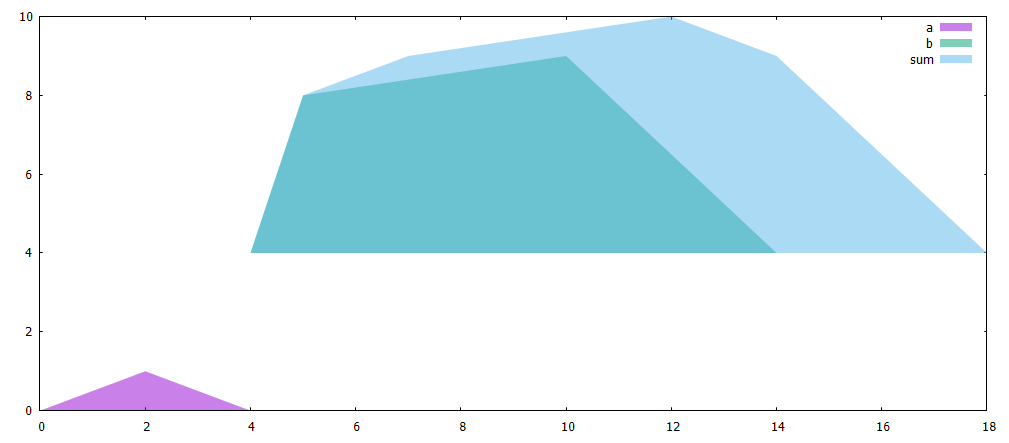
\includegraphics[width=1.0\textwidth]{minkowski_sum}
  
  \end{frame}
  
  %------------------------------------------------
  
  \begin{frame}
    \frametitle{Геометрическая разность}
    
    Операция обратная алгебраической сумме

    \begin{equation}
      A \ominus B =  \{ x | x + B \subseteq A \} 
    \end{equation}

    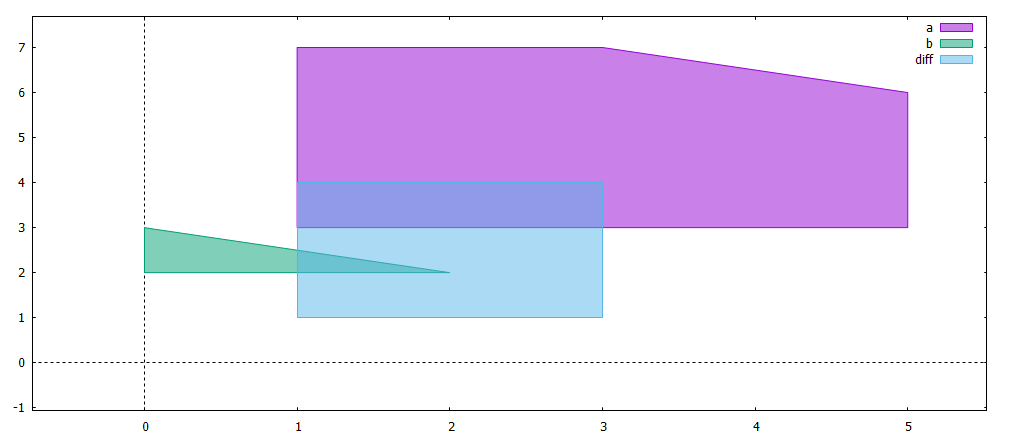
\includegraphics[width=1.0\textwidth]{geom_diff}

  \end{frame}
  
  %------------------------------------------------
  
  \begin{frame}
    \frametitle{Пример игры}
  
    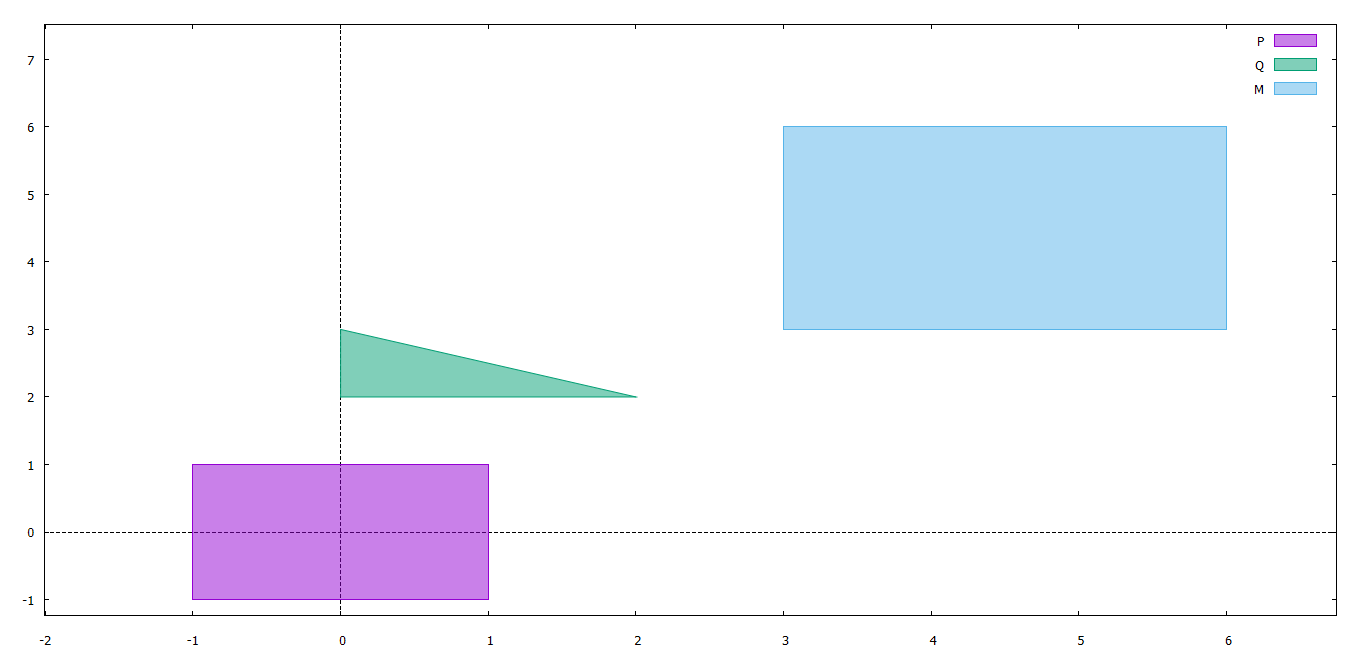
\includegraphics[width=1.0\textwidth]{game}

  \end{frame}
  
  %------------------------------------------------

  \begin{frame}
    \frametitle{Сечения стабильного моста}
  
    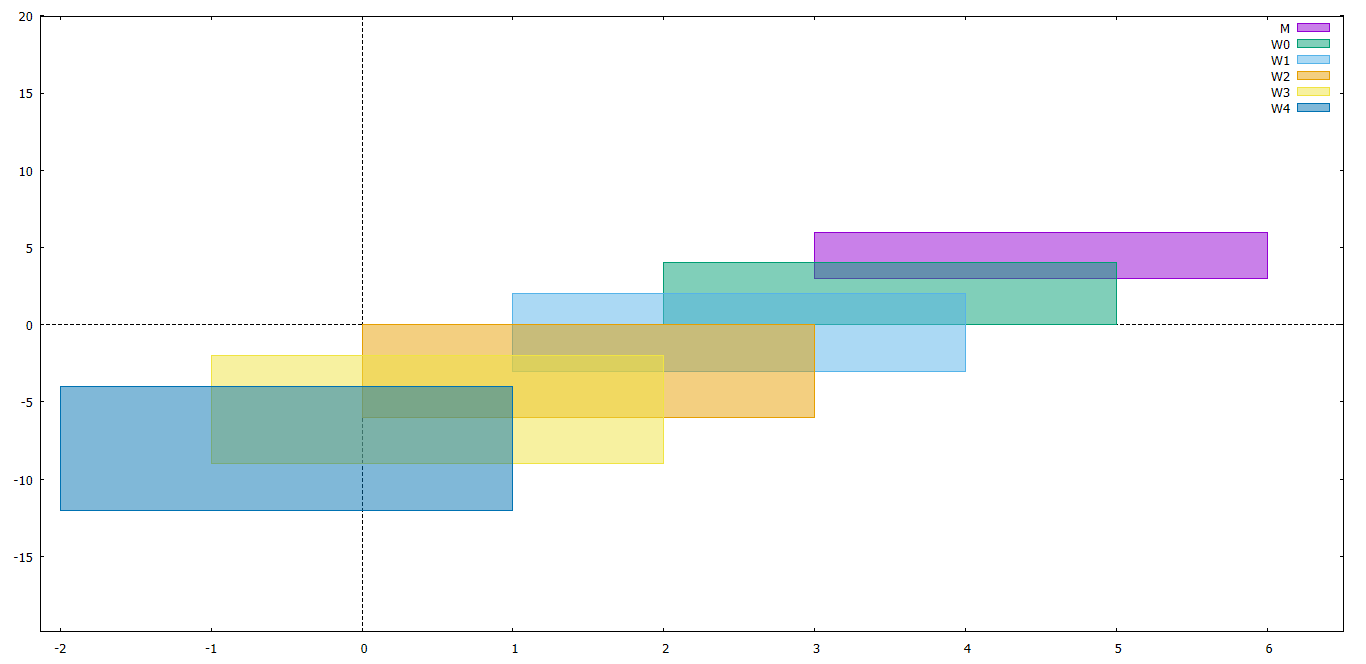
\includegraphics[width=1.0\textwidth]{bridge}
    
  \end{frame}

  %------------------------------------------------ 
  \begin{frame}
  \Huge{\centerline{Спасибо за внимание}}
  \end{frame}
  
  %----------------------------------------------------------------------------------------
  
  \end{document}